% Sección de metodología del proyecto (Entregables 1 a 3). Se incluye desde main.tex. Cifras tomadas del
% Entregable 3 (artículo, libro de Jupyter y resultados/) sin volver a ejecutar ningún experimento.
\section{Metodología}
\label{sec:metodologia}

Esta sección describe el problema, los datos y su preparación, el modelo propuesto, su entrenamiento, los
modelos de referencia, el protocolo de comparación y el diseño del estudio de ablación; las cifras de
desempeño se reservan para la sección de resultados.

\subsection{Formulación del problema y notación}
\label{sec:formulacion}

Una \emph{fintech} quiere ordenar a sus clientes por riesgo de abandono para concentrar en ellos una campaña
de retención de capacidad limitada. Cada cliente $i$ se describe con un vector $\bm{x}_i \in \X \subset \R^{p}$
($p = 78$ columnas tras el preprocesamiento) y con un puntaje de propensión $s_i \in [0{,}114;\ 0{,}501]$, la
columna \cp\ del conjunto, que nunca vale 0 ni 1: no es un evento observado sino un puntaje. Se abordan dos
tareas supervisadas sobre los mismos predictores. En \textbf{regresión} se busca $f_R: \X \to \R$ que
minimice el error cuadrático medio del puntaje, con la raíz de ese error (RMSE) como métrica principal. En
\textbf{clasificación} se define el \emph{riesgo alto} como el cuarto superior del puntaje,
$z_i = \mathbb{1}[\,s_i > \tau\,]$, con $\tau$ el percentil 75 de $s$ estimado solo en el entrenamiento
($\tau = 0{,}3927$; 24,6~\% de positivos), y se busca $f_C: \X \to [0, 1]$ que minimice la entropía cruzada
ponderada
\begin{equation}
  \mathcal{L}_C = -\frac{1}{n}\sum_{i=1}^{n} w_i \big[\, z_i \ln \hat{p}_i + (1 - z_i) \ln (1 - \hat{p}_i) \,\big],
  \qquad
  \mathcal{L}_R = \frac{1}{n}\sum_{i=1}^{n} (s_i - \hat{s}_i)^2,
  \label{eq:perdidas}
\end{equation}
donde $\hat{p}_i = f_C(\bm{x}_i)$, $\hat{s}_i = f_R(\bm{x}_i)$ y $w_i$ son pesos de clase opcionales
(sección~\ref{sec:modelo}). La métrica principal de clasificación es el área bajo la curva ROC (AUC), porque
no depende del umbral ni de la prevalencia y mide lo que necesita la campaña: ordenar a los clientes por
riesgo. La comparación con la entrega anterior usa su misma etiqueta, el riesgo alto como la mitad superior
del puntaje ($\tau = 0{,}354$, 49,9~\% de positivos en la prueba), para que las cifras sean comparables. La
tabla~\ref{tab:notacion} resume la notación.

\begin{table}[t]
  \centering\small
  \caption{Notación principal de la sección.}
  \label{tab:notacion}
  \begin{tabular}{@{}>{\raggedright\arraybackslash}p{0.2\linewidth} >{\raggedright\arraybackslash}p{0.74\linewidth}@{}}
    \toprule
    Símbolo & Significado \\
    \midrule
    $\bm{x}_i \in \R^{p}$ & predictores del cliente $i$ tras el preprocesamiento ($p = 78$) \\
    $s_i$, $\hat{s}_i$ & puntaje de propensión \cp\ y su predicción (regresión) \\
    $z_i$, $\hat{p}_i$, $\tau$ & etiqueta de riesgo alto, probabilidad predicha y umbral de riesgo alto (percentil 75 del entrenamiento; la mediana en la comparación con la entrega anterior) \\
    $f_C$, $f_R$ & predictores de clasificación y de regresión que minimizan la ecuación~\eqref{eq:perdidas} \\
    $\ell$, $\hat{u}_i$ & pérdida de un cliente en la escala del enlace y predicción acumulada en esa escala (\emph{boosting}) \\
    $n$, $n_{\mathrm{te}}$ & clientes de entrenamiento (38.978) y de prueba (9.745) \\
    $w_i$ & peso de clase por observación, $n / (2 n_{z_i})$ con ponderación y 1 sin ella \\
    $f_j$, $f_{jk}$, $K$ & funciones de forma de una variable y de un par, y número de pares de la EBM \\
    $B$, $\eta$, $L$, $m$ & bolsas externas, tasa de aprendizaje, hojas por árbol y mínimo por hoja de la EBM \\
    $g$ & función de enlace: logit en clasificación, identidad en regresión \\
    $M$, $\mathrm{bins}$ & rondas de \emph{boosting} y número de intervalos de discretización \\
    $\auc$, $\rmse$ & métricas principales de clasificación y de regresión \\
    \bottomrule
  \end{tabular}
\end{table}

\subsection{Datos, análisis exploratorio y preprocesamiento}
\label{sec:datos}

\paragraph{Fuente y tamaño.}
Se usa COFINFAD, \emph{Colombian Fintech Financial Analytics Dataset} \citep{cofinfad2025}, publicado en
Mendeley Data (DOI 10.17632/mhb4zn3258.1, licencia CC~BY~4.0). Describe a los clientes de una \emph{fintech}
colombiana durante 2023 en dos tablas: una con un registro por cliente (48.723 filas y 54 columnas: perfil,
tenencia de productos, uso digital, satisfacción, resúmenes transaccionales y los objetivos) y otra con el
detalle de 3.159.157 transacciones.

\paragraph{ETL y preprocesamiento.}
La auditoría del detalle no encontró montos no positivos, fechas nulas ni transacciones huérfanas, y eliminó
102 transacciones duplicadas. De él se derivaron doce variables de comportamiento por cliente (número de
transacciones; monto total, medio y mediano; recencia; días y meses activos; volatilidad del monto y
proporción de cada tipo de transacción), ninguna de las cuales usa el objetivo. Se eliminaron diecisiete
columnas con la evidencia de la tabla~\ref{tab:etl}, y el único faltante que se conserva,
\texttt{credit\_utilization\_ratio} (37,5~\% de los clientes), falta exactamente cuando el cliente no tiene
tarjeta de crédito: no es un dato perdido sino un \emph{no aplica}, y se imputa con cero. Las categóricas se
codifican con indicadoras (descartando un nivel) y las numéricas y booleanas se estandarizan; esas
transformaciones, y el sobremuestreo cuando lo hay, se ajustan dentro de cada pliegue de cada validación
cruzada. Los atípicos de los predictores no se recortan: las variables de conteo y transaccionales tienen
colas largas (el 18~\% de los clientes queda fuera de 1,5 rangos intercuartílicos en las transacciones
fallidas y entre el 9 y el 12~\% en frecuencia, número y montos), pero son clientes muy activos, no errores,
y los árboles son invariantes a transformaciones monótonas.
El conjunto final tiene 48 predictores (32 numéricos, 9 categóricos y 7 booleanos), que el preprocesamiento
convierte en $p = 78$ columnas.

\begin{table}[t]
  \centering\small
  \caption{Columnas eliminadas en el ETL y razón de cada decisión.}
  \label{tab:etl}
  \begin{tabular}{@{}>{\raggedright\arraybackslash}p{0.34\linewidth} >{\raggedright\arraybackslash}p{0.6\linewidth}@{}}
    \toprule
    Columnas & Razón \\
    \midrule
    identificador del cliente & sin valor predictivo \\
    \ap & fuga de información: el puntaje se construyó a partir de ella (párrafo siguiente y figura~\ref{fig:objetivo}) \\
    valor del cliente y su segmento & son el segundo objetivo del proyecto \\
    cuatro resúmenes transaccionales & duplican a otras columnas (dos con los mismos valores repartidos entre clientes distintos; dos con $r = 1{,}000$ con la frecuencia de transacciones) \\
    dos fechas & duplican a otras fechas \\
    tres fechas (\texttt{last\_survey\_date}, \texttt{first\_tx}, \texttt{last\_tx}) & sin señal ($\eta^2 = 0{,}0087$, $0{,}0046$ y $0{,}0044$) \\
    \texttt{nps\_score} & colinealidad con la satisfacción ($r = 0{,}917$) \\
    \texttt{occupation} & 35 niveles sin señal ($\eta^2 = 0{,}0010$) \\
    dos columnas de texto & 50~\% y 33~\% de valores ausentes sin mecanismo ni señal \\
    \bottomrule
  \end{tabular}
\end{table}

\paragraph{Variable objetivo y hallazgos del análisis exploratorio.}
El puntaje tiene una distribución unimodal y asimétrica a la izquierda (asimetría $-0{,}61$;
figura~\ref{fig:objetivo}, izquierda), sin atípicos que tratar (el 1,0~\% del entrenamiento queda bajo la
cerca inferior de Tukey, 0,168, y ninguno sobre la superior; son puntajes válidos y no se recortan). Tres
hallazgos condicionan el modelado. Primero, la edad solo toma seis valores (29, 30, 44, 45, 59 y 60 años, con
unos 8.120 clientes cada uno): el conjunto se generó por tres cohortes y el archivo está ordenado por bloques
que las siguen, en los que la proporción de riesgo alto va del 8 al 46~\%. Segundo, \ap\ es la variable más
correlacionada con el puntaje ($r = -0{,}876$; explica el 76,8~\% de su varianza) y su media desciende en
una escalera de saltos casi idénticos ($-0{,}0498$, $-0{,}0496$, $-0{,}0508$ y $-0{,}0496$; figura
\ref{fig:objetivo}, derecha). Un paso constante es la firma de una regla de generación, no de una asociación
empírica: un modelo que conoce esa variable recupera la fórmula del puntaje en lugar de predecir la fuga, así
que se excluye como predictor por fuga de información \citep{kaufman2012leakage} y se mide el techo que deja
su ausencia (sección~\ref{sec:protocolo}). Tercero, sin ella la señal se concentra en cuatro variables, con
correlaciones de Spearman de $-0{,}279$ (frecuencia de uso de la aplicación), $+0{,}210$ (edad), $-0{,}190$
(satisfacción) y $-0{,}164$ (satisfacción de base); las doce transaccionales no aportan ($|\rho| \leq 0{,}018$),
y las relaciones no son lineales: la frecuencia de uso reduce el riesgo con fuerza al principio y luego se
aplana, la satisfacción lo baja por escalones y la satisfacción de base sigue una curva en S. Las dos
satisfacciones miden aspectos parecidos ($\rho = 0{,}83$) y se dejan a la regularización de cada modelo.

\begin{figure}[t]
  \centering
  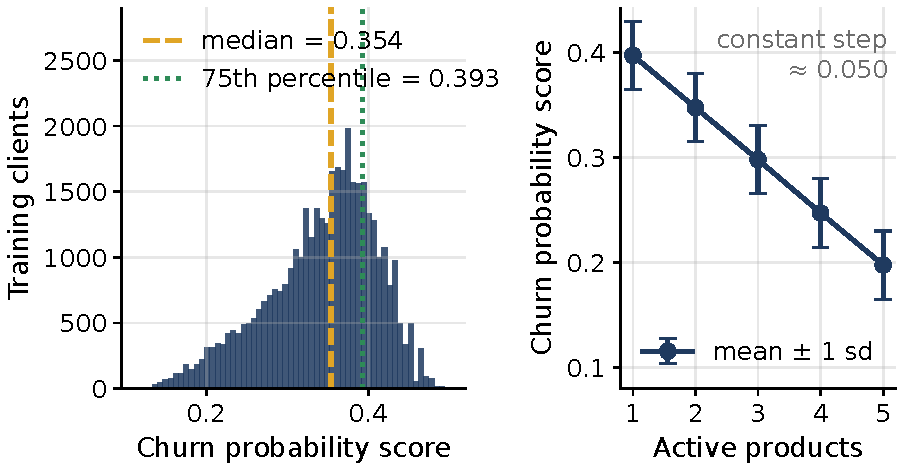
\includegraphics[width=\linewidth]{fig_target.pdf}
  \caption{Izquierda: distribución del puntaje \cp\ en el entrenamiento con los umbrales de la mediana
  (etiqueta de la entrega anterior) y del percentil 75 (etiqueta de este trabajo). Derecha: media y desviación
  del puntaje por número de productos activos; el paso constante delata la regla con la que se generó el
  puntaje y justifica excluir esa variable.}
  \label{fig:objetivo}
\end{figure}

\paragraph{Particiones y control de fugas.}
La partición es 80/20 por índices con semilla 42 ($n = 38.978$ clientes de entrenamiento y
$n_{\mathrm{te}} = 9.745$ de prueba),
aleatoria y no por posición porque el archivo está ordenado por cohortes, y se hace antes de calcular
cualquier estadístico del objetivo: el umbral $\tau$ se estima solo con el entrenamiento y la prueba no se
toca hasta la evaluación final. Se eligió la etiqueta del percentil 75 porque con la mediana las clases
quedan al 50~\% por construcción y el balanceo no tiene nada que hacer. Toda selección de hiperparámetros se
hace dentro del entrenamiento con validación cruzada anidada (sección~\ref{sec:entrenamiento}), y las
pruebas que dependen del orden de las filas se calculan en el orden original del archivo, que induce
dependencia entre vecinos.

\subsection{Modelo propuesto}
\label{sec:modelo}

\paragraph{Idea central.}
Se propone una \emph{Explainable Boosting Machine} (EBM) \citep{lou2012intelligible,lou2013ga2m}, en la
implementación \texttt{interpret} \citep{nori2019interpretml}: un modelo aditivo generalizado con
interacciones por pares (GA$^2$M) cuyas funciones de forma se aprenden por \emph{boosting} cíclico de árboles
de pocas hojas. Reúne dos propiedades que rara vez van juntas: la flexibilidad del \emph{boosting} para
representar efectos no lineales y la legibilidad de un modelo aditivo, en el que la predicción es
literalmente la suma de curvas que se pueden graficar y auditar. No forma parte de los modelos del curso. Para
adaptarla al problema se implementa la ponderación de clases mediante pesos por observación y se aplica una
búsqueda de hiperparámetros multi-fidelidad; la figura~\ref{fig:ebm} muestra la arquitectura.

\begin{figure}[tbp]
  \centering
  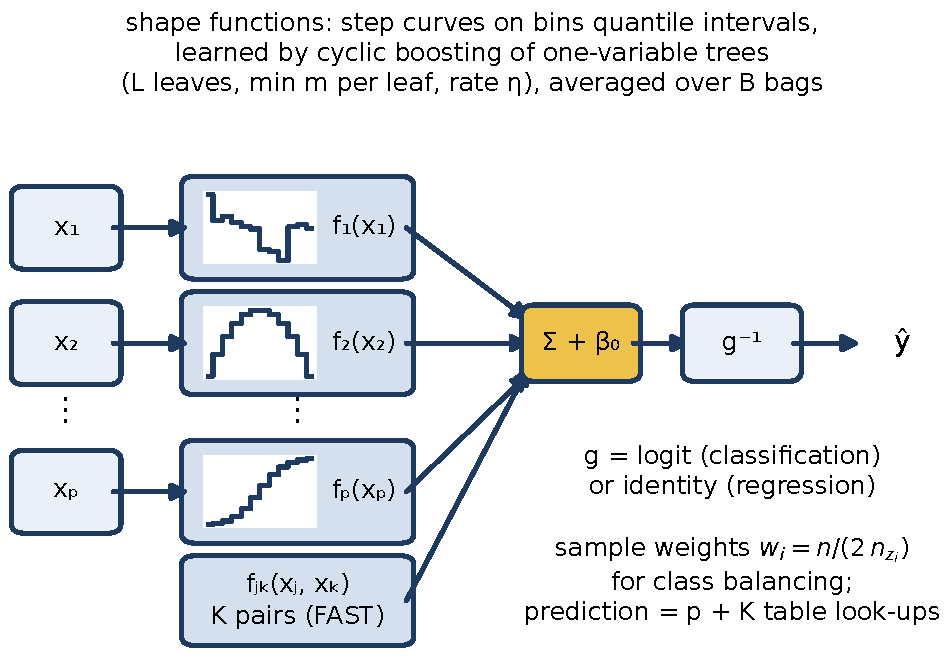
\includegraphics[width=\linewidth]{fig_ebm_architecture.pdf}
  \caption{Arquitectura del modelo propuesto: cada predictor aporta una función de forma escalonada, las
  $K$ interacciones por pares aportan una superficie cada una, la suma pasa por el enlace inverso y da la
  predicción. Cada función se aprende por \emph{boosting} cíclico de árboles de una variable y se promedia
  sobre $B$ bolsas externas.}
  \label{fig:ebm}
\end{figure}

\paragraph{Formulación.}
La EBM modela
\begin{equation}
  g\big(\E[\,y \mid \bm{x}\,]\big) = \beta_0 + \sum_{j=1}^{p} f_j(x_j) + \sum_{(j,k) \in \mathcal{I}} f_{jk}(x_j, x_k),
  \label{eq:ebm}
\end{equation}
donde $y$ es $z$ o $s$ según la tarea, $g$ es el enlace logit en clasificación y la identidad en regresión,
$f_j$ son funciones de forma unidimensionales y $\mathcal{I}$ es un conjunto de $K$ pares elegido con el
algoritmo FAST \citep{lou2013ga2m}. A diferencia de un GAM con \emph{splines}, cada $f_j$ es una función
escalonada sobre una discretización de $x_j$ en $\mathrm{bins}$ intervalos por cuantiles, aprendida por
\emph{boosting} cíclico: en cada ronda $r$ se recorren las $p$ variables en orden y, para cada una, se ajusta
un árbol de regresión $h$ de $L$ hojas y al menos $m$ observaciones por hoja \emph{solo sobre esa variable} al
gradiente negativo de la pérdida en la predicción acumulada $\hat{u}_i$ (en la escala de $g$), y se añade
escalado por una tasa $\eta$ pequeña:
\begin{equation}
  f_j^{(r+1)}(x_j) = f_j^{(r)}(x_j) + \eta\, h_j^{(r)}(x_j),
  \qquad
  h_j^{(r)} = \arg\min_{h} \sum_{i=1}^{n} w_i \big( \varrho_i^{(r)} - h(x_{ij}) \big)^2,
  \label{eq:boosting}
\end{equation}
con $\ell(y_i, \hat{u}_i)$ el término del cliente $i$ en la pérdida de la ecuación~\eqref{eq:perdidas}, escrito
en la escala del enlace ($\hat{u}_i = \operatorname{logit} \hat{p}_i$ en clasificación y $\hat{u}_i = \hat{s}_i$ en
regresión), y $\varrho_i^{(r)} = -\partial \ell(y_i, \hat{u}_i^{(r)}) / \partial \hat{u}_i^{(r)}$ su gradiente
negativo. La tasa baja hace que el orden de las variables no importe y reparte la señal compartida entre variables
correlacionadas. El procedimiento se repite sobre $B$ submuestras (bolsas externas) y las funciones se
promedian, $f_j = \frac{1}{B}\sum_b f_j^{(b)}$, lo que reduce su varianza y da un intervalo para cada tramo.
La predicción de un cliente es una suma de $p + K$ búsquedas en tablas.

\paragraph{Adaptaciones.}
La librería no ofrece ponderación de clases; se implementó un envoltorio que, cuando la corrida usa
ponderación, pasa a la EBM pesos por observación
\begin{equation}
  w_i = \frac{n}{2\, n_{z_i}},
  \label{eq:pesos}
\end{equation}
con $n_{z_i}$ el número de clientes de la clase de $i$, de modo que la pérdida ponderada
$\sum_i w_i\, \ell(y_i, \hat{u}_i)$ de la ecuación~\eqref{eq:perdidas} equivale a la ponderación balanceada de scikit-learn que reciben los modelos de
referencia. La búsqueda de hiperparámetros es multi-fidelidad: durante la búsqueda cada configuración se
evalúa con $B = 2$ bolsas y el modelo que se mide en el bucle externo y se guarda se reajusta con $B = 8$;
como las bolsas promedian pero no cambian la forma de cada función, el orden de las configuraciones se
conserva, supuesto que se comprueba empíricamente (sección~\ref{sec:ablacion}). El espacio de búsqueda es
$\eta \in [0{,}008;\ 0{,}1]$ (escala logarítmica; por debajo de 0,008 cada ajuste tarda el doble),
$L \in \{2, 3, 4\}$, $m \in [2, 200]$ (log), $K \in \{0, \dots, 20\}$ (0 es un GAM puro) y
$\mathrm{bins} \in [64, 1024]$ (log), con una rejilla de 36 puntos. El algoritmo~\ref{alg:ebm} resume el
entrenamiento.

\begin{algorithm}[t]
  \caption{Entrenamiento de la EBM con bolsas externas, pesos de clase y multi-fidelidad.}
  \label{alg:ebm}
  \begin{algorithmic}[1]
    \Require entrenamiento $\{(\bm{x}_i, y_i)\}_{i=1}^{n}$; pesos $w_i$ (1, o la ecuación~\eqref{eq:pesos} con ponderación); bolsas $B$; tasa $\eta$; hojas $L$; mínimo por hoja $m$; pares $K$; intervalos $\mathrm{bins}$
    \Ensure $\beta_0$, funciones de forma $f_j$ y $f_{jk}$
    \State discretizar cada $x_j$ en $\mathrm{bins}$ intervalos por cuantiles (una sola vez)
    \For{$b = 1, \dots, B$}
      \State tomar una submuestra de entrenamiento y reservar el resto como validación de la bolsa
      \State $f_j^{(b)} \gets 0$ para todo $j$;\quad $\hat{u}_i \gets \beta_0$ (logit de la media ponderada, o la media)
      \While{la pérdida ponderada en la validación de la bolsa mejore (parada temprana)}
        \For{$j = 1, \dots, p$} \Comment{ciclo sobre las variables}
          \State $\varrho_i \gets -\partial \ell(y_i, \hat{u}_i) / \partial \hat{u}_i$ para todo $i$
          \State ajustar un árbol $h$ de $L$ hojas y mínimo $m$ sobre $x_j$ al residuo $\varrho$ con pesos $w_i$
          \State $f_j^{(b)} \gets f_j^{(b)} + \eta\, h$;\quad $\hat{u}_i \gets \hat{u}_i + \eta\, h(x_{ij})$
        \EndFor
      \EndWhile
      \State elegir con FAST los $K$ pares $(j, k)$ que más reducen el residuo y repetir el ciclo sobre ellos con los $f_j^{(b)}$ fijos
    \EndFor
    \State $f_j \gets \frac{1}{B}\sum_b f_j^{(b)}$ y $f_{jk} \gets \frac{1}{B}\sum_b f_{jk}^{(b)}$, centradas;\quad $\beta_0 \gets$ media de las predicciones
    \State \textbf{búsqueda:} evaluar cada configuración con $B = 2$ en la validación interna; \textbf{modelo final:} reajustar la ganadora con $B = 8$
  \end{algorithmic}
\end{algorithm}

\paragraph{Justificación de cada componente.}
El análisis exploratorio muestra que la señal está en pocas variables con efectos no lineales y que los
pares de predictores son casi independientes: esa es exactamente la hipótesis aditiva de la
ecuación~\eqref{eq:ebm}, que representa escalones, mesetas y curvas en S sin interacciones profundas. Frente
a los modelos lineales, la EBM gana flexibilidad por variable; frente a XGBoost y Random Forest, restringe el
espacio de hipótesis a sumas de funciones de una variable y de pocos pares, lo que reduce la varianza en un
problema con 39.000 filas y una señal débil. Las bolsas externas estabilizan las curvas como el
\emph{bagging} de un bosque. Los pesos de la ecuación~\eqref{eq:pesos} ponen a la EBM en igualdad de
condiciones con las referencias cuando la corrida usa ponderación de clases, y la multi-fidelidad hace viable
una búsqueda cuyo coste crece con $B$. Finalmente, el modelo no necesita un explicador: cada $f_j$ es la
explicación.

\paragraph{Complejidad computacional.}
El entrenamiento recorre las $p$ variables en cada ronda: cuesta $O(B\, M\, p\, (n + \mathrm{bins}))$ para
$M$ rondas, con $n = 38.978$, $p = 78$ y $B = 8$ en el modelo final; la inferencia cuesta $O(p + K)$
búsquedas en tablas por cliente. Los parámetros del modelo son los valores de las funciones escalonadas: a
lo sumo $p \cdot \mathrm{bins}$ números para las funciones de una variable y $K \cdot \mathrm{bins}^2$ para
los pares; en el modelo final ($K = 0$, $\mathrm{bins} = 1024$) son a lo sumo $32 \cdot 1024 + 46 \cdot 2 \approx
32.900$ valores, porque las 46 columnas indicadoras y booleanas solo tienen dos intervalos, y el modelo
serializado ocupa 1,5~MB frente a los 44~MB de un bosque de 300 árboles. Medido en el equipo de la sección~\ref{sec:entrenamiento},
el ajuste final tarda 26,7~s en clasificación y 31,8~s en regresión, la inferencia sobre los 9.745 clientes
de prueba 0,067 y 0,054~s, y la corrida anidada completa 18,7 y 26,6 minutos.

\paragraph{Qué es nuevo y qué se reutiliza.}
Se reutilizan la EBM tal como la publican \citet{lou2013ga2m} y su implementación \texttt{interpret-core}
\citep{nori2019interpretml}, el conjunto de datos y las decisiones de depuración de las entregas anteriores
(columnas eliminadas y variables transaccionales derivadas), revalidadas aquí con la partición hecha antes de
cualquier estadístico del objetivo, y el pipeline combinatorio y el protocolo estadístico de la guía del curso. Lo nuevo es la
elección y la adaptación del modelo a este problema: no se vio en el curso, la ponderación de clases por
observación y la búsqueda multi-fidelidad no existen en la librería, y la EBM se integra en el mismo
pipeline, con las mismas reglas y el mismo presupuesto, que los modelos de referencia, de modo que la
comparación es justa.

\subsection{Entrenamiento y optimización}
\label{sec:entrenamiento}

\paragraph{Optimización.}
La EBM se ajusta por el \emph{boosting} cíclico del algoritmo~\ref{alg:ebm}, con parada temprana por bolsa
sobre su validación interna y sin lotes ni épocas en el sentido de las redes. No tiene penalización explícita:
la regularizan la tasa $\eta$ baja, el mínimo $m$ por hoja, las $L \leq 4$ hojas, la parada temprana y el
promedio sobre $B$ bolsas. Sus hiperparámetros finales, elegidos por el protocolo de la
sección~\ref{sec:protocolo}, aparecen en la tabla~\ref{tab:espacios}. Los
modelos de referencia usan el solucionador de su implementación: liblinear para la logística, Cholesky para
Ridge, descenso por coordenadas para Lasso, el método \texttt{hist} para XGBoost y el primal con pérdida de
bisagra al cuadrado para el SVM lineal, elegidos tras medir su coste.

\begin{table}[t]
  \centering\scriptsize\setlength{\tabcolsep}{3pt}
  \caption{Espacios de búsqueda (rejilla de Grid Search, igual al presupuesto de los otros tres métodos) e
  hiperparámetros finales de la mejor combinación en clasificación (Clas.) y en regresión (Regr.).}
  \label{tab:espacios}
  \begin{tabular}{@{}>{\raggedright\arraybackslash}p{0.13\linewidth} r >{\raggedright\arraybackslash}p{0.42\linewidth} >{\raggedright\arraybackslash}p{0.33\linewidth}@{}}
    \toprule
    Modelo & Rejilla & Espacio de búsqueda & Hiperparámetros finales \\
    \midrule
    EBM (propuesto) & 36 & $\eta \in [0{,}008;\ 0{,}1]$ (log); $L \in \{2, 3, 4\}$; $m \in [2, 200]$ (log); $K \in \{0, \dots, 20\}$; $\mathrm{bins} \in [64, 1024]$ (log) & Clas.: $K = 0$, $\eta = 0{,}008$, $L = 2$, $m = 100$, $B = 8$, $\mathrm{bins} = 1024$ (valor por defecto; la rejilla no lo recorre). Regr.: $K = 0$, $\eta = 0{,}008$, $L = 3$, $m = 20$, $B = 8$, $\mathrm{bins} = 1024$ \\
    k-NN & 32 & $k \in [5, 600]$ (entero, log); pesos uniformes o por distancia; $q \in \{1, 2\}$ & Clas.: $k = 600$, distancia, $q = 1$. Regr.: $k = 80$, distancia, $q = 1$ \\
    Naive Bayes & 30 & \texttt{var\_smoothing} $\in [10^{-11}, 10^{-3}]$ (log) & Clas.: $10^{-3}$ \\
    Regresión logística & 30 & $C \in [10^{-3}, 10^{2}]$ (log); penalización $\in \{\mathrm{L1}, \mathrm{L2}\}$ & Clas.: $C = 0{,}0563$, L1 \\
    Ridge / Lasso & 30 & $\alpha \in [10^{-3}, 10^{5}]$ / $[10^{-6}, 10^{-1}]$ (log) & Regr.: $\alpha = 613{,}9$ / $1{,}09 \cdot 10^{-4}$ \\
    Árbol de decisión & 48 & profundidad $\in [3, 30]$; mínimo por hoja $\in [1, 300]$ (log); $\gamma \in [10^{-6}, 10^{-2}]$ (Clas.) o $[10^{-8}, 10^{-4}]$ (Regr.) (log); Gini o entropía (Clas.) & Clas.: 22; 7; $3{,}9 \cdot 10^{-4}$; Gini. Regr.: 13; 101; $1{,}8 \cdot 10^{-6}$ \\
    Random Forest & 36 & profundidad $\in [4, 40]$; variables por partición $\in \{\sqrt{p}, \log_2 p, 0{,}3, 0{,}5\}$; mínimo por hoja $\in [1, 100]$ (log); $T = 100$ en la búsqueda y 300 en el final & Clas.: 32; 0,5; 11. Regr.: 8; 0,5; 50 \\
    XGBoost & 32 & árboles $\in [100, 1000]$ (log); profundidad $\in [2, 10]$; tasa $\in [10^{-3}, 0{,}3]$ (log); submuestreo de filas y de columnas $\in [0{,}5;\ 1]$; penalización L2 de las hojas $\lambda \in [0{,}01;\ 10]$ (log); peso mínimo por hoja $\in [1, 50]$ (log) & Clas.: 145; 6; 0,0033; 0,81; 0,97; 0,88; 11. Regr.: 512; 2; 0,024; 0,80; 0,73; 0,22; 31 \\
    SVM / SVR lineal & 30 & $C \in [10^{-4}, 10^{2}]$ (Clas.) o $[10^{-3}, 10^{2}]$ (Regr.) (log); $\varepsilon \in [10^{-4};\ 0{,}05]$ (log, Regr.) & Clas.: $C = 0{,}0011$. Regr.: $C = 46{,}4$, $\varepsilon = 3{,}8 \cdot 10^{-4}$ \\
    \bottomrule
  \end{tabular}
\end{table}

\paragraph{Búsqueda de hiperparámetros.}
Cada corrida es una validación cruzada anidada \citep{cawley2010overfitting}: un bucle externo de 5
pliegues (estratificados en clasificación, los mismos para todos los modelos) produce la única métrica que
se reporta, y dentro de cada pliegue externo un bucle interno de 3 pliegues elige los hiperparámetros con uno
de los cuatro métodos de la tabla~\ref{tab:optimizadores}, que reciben el mismo presupuesto: tantas
evaluaciones como puntos tiene la rejilla del modelo (entre 30 y 48). Al terminar, la misma búsqueda se
repite sobre todo el entrenamiento y el ganador se reajusta con él: es el modelo final, que toca la prueba
una sola vez. El mejor puntaje interno se guarda para medir el optimismo de selección, pero nunca se reporta.

\begin{table}[t]
  \centering\small
  \caption{Los cuatro métodos de búsqueda de hiperparámetros, con el mismo presupuesto por modelo.}
  \label{tab:optimizadores}
  \begin{tabular}{@{}>{\raggedright\arraybackslash}p{0.19\linewidth} >{\raggedright\arraybackslash}p{0.38\linewidth} >{\raggedright\arraybackslash}p{0.37\linewidth}@{}}
    \toprule
    Método & Cómo propone cada evaluación & Parámetros \\
    \midrule
    Grid Search & recorre la rejilla del modelo & puntos de la rejilla: de 30 a 48 \\
    Random Search & muestrea el espacio tipado & escala logarítmica para $C$, $\alpha$ y las tasas; enteros en escala logarítmica para vecinos y tamaños de hoja \\
    Bayesiana (TPE de Optuna \citep{akiba2019optuna}) & modela las densidades de las configuraciones mejores y del resto y propone el máximo de su cociente & 10 ensayos aleatorios de arranque; cuantil 0,10 para separar las mejores \\
    Genética (DEAP) & genes en $[0, 1]$, selección por torneo, cruce uniforme, mutación gaussiana y elitismo & torneo de 3; cruce con probabilidad 0,5 por gen, aplicado con 0,6; mutación con $\sigma = 0{,}15$ y probabilidad 1/(número de hiperparámetros) por gen, aplicada con 0,3; población entre 4 y 12 (presupuesto/4) \\
    \bottomrule
  \end{tabular}
\end{table}

\paragraph{Semillas, software y hardware.}
Una semilla única (42) se propaga a la partición, a cada estimador, al remuestreo, a los optimizadores y a
los \emph{bootstrap}; la sensibilidad a la semilla se mide reentrenando los modelos finales de Random
Forest, XGBoost, SVM y EBM con cinco a diez semillas y repitiendo la búsqueda del árbol con cinco semillas de
cada optimizador estocástico. El software es Python 3.13.3 con scikit-learn 1.9.1 \citep{pedregosa2011sklearn},
imbalanced-learn 0.14.2, XGBoost 3.4.1, interpret-core 0.7.8, Optuna 5.0.0 y DEAP 1.4.4, con las versiones
exactas fijadas. El equipo es un escritorio con procesador AMD de seis núcleos, 15,9~GB de memoria y una GPU
NVIDIA GeForce RTX~3050 de 6~GB (que no acelera estos modelos y solo se usó para medirlo), con Windows~11.
Las 140 corridas de la guía se ejecutaron en serie, con el equipo dedicado y el código congelado con su huella
SHA-256, y sumaron 26,9 horas; las 20 corridas de la EBM, 19,5 horas. El tiempo se reporta de tres formas:
duración de cada corrida anidada, ajuste del modelo final sobre los 38.978 clientes y tiempo de inferencia
sobre los 9.745 de prueba, estos dos como mediana de tres ajustes y cinco inferencias con el pipeline
completo.

\subsection{Modelos de referencia}
\label{sec:referencias}

\begin{sloppypar}
El modelo propuesto se compara con todos los modelos del curso en las dos tareas, en su implementación de
scikit-learn \citep{pedregosa2011sklearn} salvo XGBoost: k vecinos más cercanos, Naive
Bayes gaussiano, regresión logística con penalización L1 o L2, Ridge y Lasso,
árbol de decisión CART \citep{breiman1984cart}, Random Forest \citep{breiman2001rf}, XGBoost
\citep{chen2016xgboost} y máquinas de vectores de soporte lineales \citep{cortes1995svm}, porque el núcleo
RBF multiplica por 70 el coste del ajuste; se añaden los dos modelos de la entrega anterior, reentrenados con
sus hiperparámetros (regresión logística L1 con $C = 0{,}1$ y Lasso con $\alpha = 10^{-4}$). Todos usan las
mismas particiones, el mismo preprocesamiento y el mismo presupuesto de búsqueda que la EBM
(tabla~\ref{tab:espacios}), y cada clasificador se entrena con cuatro técnicas de balanceo: sin balanceo,
SMOTE \citep{chawla2002smote}, ADASYN y ponderación de clases con la ecuación~\eqref{eq:pesos}; el
sobremuestreo se ajusta solo con las filas de entrenamiento de cada pliegue y las combinaciones que no
aplican (k-NN con ponderación, que vota sin función de pérdida) se registran como tales. En regresión no hay
balanceo. Random Forest usa la misma multi-fidelidad que la EBM (100 árboles en la búsqueda, 300 en el modelo
final) y XGBoost pondera las clases con el cociente negativos/positivos del pliegue.
\end{sloppypar}

\subsection{Protocolo de evaluación}
\label{sec:protocolo}

\paragraph{Métricas.}
En clasificación, la métrica principal es el AUC; se reportan además el AUC-PR y, en el punto de operación
que contacta al 25~\% de clientes de mayor riesgo, la precisión, el \emph{recall}, el F1, el MCC y la exactitud
balanceada; el \emph{recall} con umbral 0,5 (la métrica secundaria de la entrega anterior) se usa para mostrar
el efecto del balanceo, y la calibración se mide con el error de calibración esperado antes y después de una
recalibración isotónica ajustada solo con predicciones fuera de pliegue. En regresión, la métrica principal es
el RMSE, con el MAE, el MAPE y el $R^2$, y los residuos se someten a las pruebas de White, BDS, Ljung-Box y de
normalidad. Las métricas principales de prueba (AUC; RMSE y $R^2$) llevan un intervalo \emph{bootstrap} BCa con
2.000 réplicas.

\paragraph{Validación.}
La validación cruzada anidada de la sección~\ref{sec:entrenamiento} produce, para cada corrida, la media y
la desviación de la métrica en los 5 pliegues externos, con las que se elige la mejor combinación de cada
modelo sin mirar la prueba, que se evalúa una sola vez con el modelo final (figura~\ref{fig:pipeline}). Como el objetivo se generó a partir de \ap, se estima además el
techo de información que deja su exclusión: el pronóstico de un oráculo (\emph{gradient boosting} de
histogramas) que sí la conoce, promediado sobre la distribución de \ap\ en el entrenamiento y evaluado en la
misma prueba.

\begin{figure}[tbp]
  \centering
  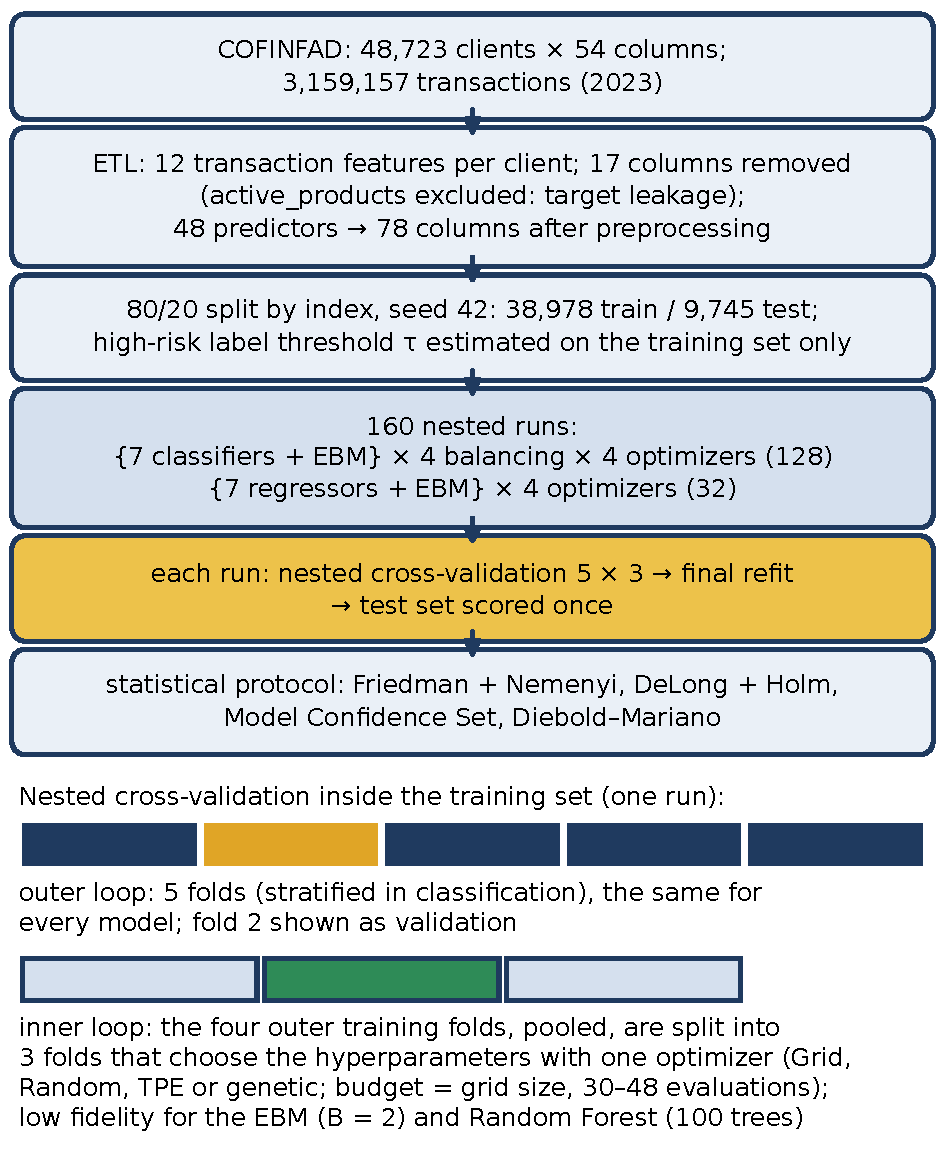
\includegraphics[width=\linewidth]{fig_pipeline_nested_cv.pdf}
  \caption{Pipeline combinatorio del estudio y validación cruzada anidada de cada corrida: el bucle externo
  de 5 pliegues produce la métrica que se reporta y el interno de 3 pliegues elige los hiperparámetros con
  uno de los cuatro optimizadores; el modelo final se reajusta con todo el entrenamiento y toca la prueba una
  sola vez.}
  \label{fig:pipeline}
\end{figure}

\paragraph{Pruebas estadísticas.}
El modelo propuesto se contrasta con cada uno de los siete modelos de referencia ($m = 7$) con $\alpha = 0{,}05$
y $p$ ajustados por Holm dentro de cada prueba. En clasificación: la $t$ pareada con varianza corregida de
\citet{nadeau2003} sobre los AUC de los 5 pliegues externos (los mismos para todos los modelos), DeLong
\citep{delong1988} sobre la prueba, McNemar exacta \citep{mcnemar1947}
sobre las clases del punto de operación y la $t$ correlacionada bayesiana \citep{benavoli2017} con una región de
equivalencia práctica de $\pm 0{,}01$ de AUC. En regresión: la $t$ corregida sobre el RMSE de los pliegues,
Diebold-Mariano \citep{diebold1995} con la corrección de Harvey-Leybourne-Newbold sobre las pérdidas cuadráticas
de la prueba, la bayesiana con región de $\pm 0{,}0005$ de RMSE y, como complemento, el \emph{Model Confidence
Set} al 90~\% \citep{hansen2011mcs} con \emph{bootstrap} estacionario, con las filas en el orden original del
archivo, organizado por bloques. Cada $p$ va con un tamaño de efecto: la diferencia de métrica con intervalo BCa,
la $d$ de Cohen y la delta de Cliff. La comparación con la entrega anterior se hace en su misma partición, su
misma etiqueta y su misma prueba, con la EBM y XGBoost afinados entre sí con el mismo procedimiento (TPE con
el presupuesto de la tabla~\ref{tab:espacios} y validación cruzada de 5 pliegues sobre el entrenamiento,
reajuste final y una sola evaluación en la prueba), y se decide con DeLong (clasificación) y Diebold-Mariano
(regresión). Los cuatro optimizadores se comparan con Friedman (Iman-Davenport) y Nemenyi \citep{demsar2006},
cuyos bloques son las combinaciones modelo $\times$ balanceo y no los pliegues de un solo conjunto, por la
métrica final y por el área bajo la curva de arrepentimiento normalizado de cada búsqueda.

\subsection{Diseño del estudio de ablación}
\label{sec:ablacion}

Cada variante cambia un solo componente del modelo propuesto y conserva el resto (particiones,
preprocesamiento, presupuesto y semilla). Hipótesis y diseño de cada variante:
\begin{enumerate}
  \item \textbf{Sin interacciones} ($K = 0$, un GAM puro) frente a la EBM con sus $K$ pares, en la
        partición y la etiqueta de la entrega anterior y decidido con DeLong sobre la prueba: la hipótesis
        aditiva basta porque la señal está en pocas variables casi independientes.
  \item \textbf{Balanceo} (sin balanceo, SMOTE, ADASYN y ponderación de clases) en las corridas anidadas de
        la EBM: no mejora el AUC, que mide el orden de los clientes, y solo desplaza el punto de operación.
  \item \textbf{Fidelidad de la búsqueda}: ocho configuraciones aleatorias evaluadas con $B = 2$ y con
        $B = 8$ en la misma validación cruzada de 3 pliegues ($\rho$ de Spearman entre ambos AUC, misma
        ganadora y ahorro de tiempo): la fidelidad baja conserva el orden y ahorra tiempo.
  \item \textbf{Optimizador} (Grid, Random, TPE y genético con el mismo presupuesto): la métrica final no
        distingue a los métodos; la eficiencia por evaluación (área de arrepentimiento, medida sobre las 140
        corridas de la guía) sí.
  \item \textbf{Semilla}: el modelo final de cada tarea se reentrena con cinco semillas (desviación de la
        métrica principal de prueba): la variabilidad por semilla es del orden de las diferencias entre los
        modelos de árboles.
\end{enumerate}

\subsection{Disponibilidad de código y datos}
\label{sec:disponibilidad}

COFINFAD es público y puede descargarse de Mendeley Data (DOI 10.17632/mhb4zn3258.1, licencia CC~BY~4.0);
una copia comprimida de las dos tablas está en la carpeta \texttt{datos} del repositorio y el código la
descomprime al cargarla. El código completo (paquete \texttt{src}, guiones de las corridas, de la comparación
con la entrega anterior y de los experimentos de cómputo), la tabla maestra con las 160 corridas, las
predicciones de prueba, los cuadernos ejecutados y el libro de Jupyter están en
\url{https://github.com/RubenEsg/Prediccion-de-fuga-de-clientes-en-fintech}; el entorno se fija con
\texttt{requirements.txt} (versiones exactas), la semilla es 42 y el hardware es el de la
sección~\ref{sec:entrenamiento}.
